\documentclass{beamer}
%\usepackage{xspace}
\usepackage{amsmath,amssymb}
\usepackage{graphicx}
%\usepackage{svg}
%\usepackage{pgfpages}
%\pgfpagesuselayout{4 on 1}[a4paper,border shrink=5mm,landscape]
%\usepackage{psfrag}
%\usepackage[usenames,dvipsnames]{xcolor}
\usepackage{braket}
\usepackage{qcircuit}
\usepackage{tikz}
\usetikzlibrary{circuits.logic.US}
\usetikzlibrary{graphs}
\usetikzlibrary{datavisualization}
\usetikzlibrary{datavisualization.formats.functions}
\usepackage{pgfplotstable}
\usepgfplotslibrary{patchplots}

\setbeamercovered{transparent}

\usetheme{Pittsburgh}
%\usetheme{default}

\setbeamertemplate{sidebar right}{}
\setbeamertemplate{footline}[frame number]
%\usefonttheme{professionalfonts}

%\usepackage{sansmathaccent}
%\usepackage{bm}

%\usepackage{unicode-math}
%%\setmainfont[SlantedFont={Latin Modern Roman Slanted},SlantedFeatures={Color=000000},
%%  SmallCapsFont={TeX Gyre Termes},SmallCapsFeatures={Letters=SmallCaps}]{XITS}
%\setmathfont[math-style=ISO,sans-style=upright]{XITS Math}
%\setmathfont[range={\mathcal,\mathbfcal}]{Latin Modern Math}

\usepackage{sfmath}

%\mathversion{sans}

\newcommand{\Tr}{\mathsf{Tr}}

\definecolor{redorange}{rgb}{1.0, .25, .25}
\definecolor{citation}{rgb}{.1, 0.8, .35}
\newcommand\emm[1]{\textcolor{redorange}{{#1}}}
\newcommand\numc[1]{\textcolor{citation}{{\bf #1}}}

%\newcommand\bm[1]{{\mbox{\boldmath $#1$}}}
\newcommand\bm[1]{{\mathbf{#1}}}
%\newcommand\bm[1]{{\bf #1}}
%\newcommand\bm[1]{\ensuremath{\boldsymbol{#1}}}
%\newcommand\bm[1]{{\textbf{\it #1}}}

\title{Quantum circuit}
\author{Ryuhei Mori}
%\institute{$\vcenter{\hbox{\includegraphics[width=30pt]{ELC_logo}}}$ Postdoctoral Fellow of ELC\\ $\vcenter{\hbox{\includegraphics[width=20pt]{titech_logo}}}$ Tokyo Institute of Technology}
\institute{Tokyo Institute of Technology}
%\date{21, Feb, 2019}



\begin{document}
\begin{frame}[plain]
\maketitle
\end{frame}



\begin{frame}{Boolean circuit}
\begin{itemize}
\setlength{\itemsep}{2em}
\item Boolean function $f\colon \{0,1\}^n\to\{0,1\}$.
\item \emm{Boolean circuit} is a model of computation of a Boolean functions which consists of logic \emm{gates}.
\item AND gate:
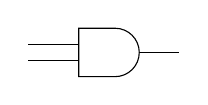
\begin{tikzpicture}[circuit logic US, baseline]
\node[and gate] (A) {};
\foreach \a in {1, 2}
  \draw (A.input \a -| -1,0) -- (A.input \a);
\draw (A.output) -- ([xshift=0.5cm]A.output);
\end{tikzpicture}
\item OR gate:
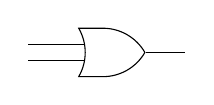
\begin{tikzpicture}[circuit logic US, baseline]
\node[or gate] (A) {};
\foreach \a in {1, 2}
  \draw (A.input \a -| -1,0) -- (A.input \a);
\draw (A.output) -- ([xshift=0.5cm]A.output);
\end{tikzpicture}
\item NOT gate:
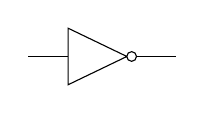
\begin{tikzpicture}[circuit logic US, baseline]
\node[not gate] (A) {};
\draw (A.input) -- ([xshift=-0.5cm]A.input);
\draw (A.output) -- ([xshift=0.5cm]A.output);
\end{tikzpicture}
\end{itemize}
\end{frame}

\begin{frame}{Universality of $\{\mathsf{AND}, \mathsf{OR},\mathsf{NOT}\}$}
\begin{theorem}
For \emm{any} Boolean function $f\colon \{0,1\}^n\to\{0,1\}$, there is a Boolean circuit with AND, OR and NOT gates computing $f$.
\end{theorem}
\begin{proof}
The proof is an induction on $n$. Theorem is trivial for $n=1$.
Assume that Theorem holds for Boolean functions $n \le k-1$.
\begin{align*}
f(x_1,\dotsc,x_k) = (x_k \wedge f(x_1,\dotsc,x_{k-1}, 1)) \vee (\overline{x_k} \wedge f(x_1,\dotsc,x_{k-1}, 0)).
\end{align*}
\end{proof}
\end{frame}

\begin{frame}{Size of Boolean circuits}
Size of Boolean circuit $:=$ \# of \emm{AND/OR gates} in the Boolean circuit.

Let $C(f)$ be a smallest size of Boolean circuit computing $f\colon\{0,1\}^n\to\{0,1\}$.

Let $s(n) := \max_{f\colon\{0,1\}^n\to\{0,1\}} C(f)$.

\begin{align*}
f(x_1,\dotsc,x_n) = (x_n \wedge f(x_1,\dotsc,x_{n-1}, 1)) \vee (\overline{x_n} \wedge f(x_1,\dotsc,x_{n-1}, 0))
\end{align*}
\begin{align*}
s(n) &\le c + 2 s(n-1)\\
\frac{s(n)}{2^n} &\le \frac{c}{2^n} + \frac{s(n-1)}{2^{n-1}}\\
&\le c \left(\frac1{2^n} + \frac1{2^{n-1}} + \dotsb \frac12\right) + s(0) \le c + s(0)
\end{align*}
\begin{center}
\begin{equation*}
s(n) = O(\emm{2^n}).
\end{equation*}
\end{center}
\end{frame}

\begin{frame}{Lower bound of size of Boolean circuits}
\emm{The number of Boolean functions} with $n$ variables is $2^{2^n}$.

\vspace{1em}
\emm{The number of Boolean circuits} of size $s$ is at most
\begin{equation*}
%\left(8\binom{n+s+2}{2}\right)^s
%\le (4(n+s)^2)^{s}.
(8(n+s)^2)^{s}.
\end{equation*}

This means
\begin{align*}
& (8(n+s(n))^2)^{s(n)}\ge 2^{2^n} \\
\iff& {s(n)}\log(8(n+s(n))^2)\ge 2^n\\
\Longrightarrow&\, s(n)\ge \frac{2^n}{3n} \quad \text{ for sufficiently large } n.
\end{align*}

\small
In fact, $s(n) = \frac{2^n}{n}(1+o(1))$.
\end{frame}

\begin{frame}{Quantum circuit}
\begin{itemize}
\setlength{\itemsep}{1.5em}
%\item Unitary operator $U\in \mathcal{L}(\mathbb{C}^{2^n})$.
\item \emm{Quantum circuit} is a model of computation of Boolean functions which consists of \emm{quantum gates}.
\item Single qubit gate: $X$ gate, $Y$ gate, $Z$ gate, $H$ gate, $S:=\begin{bmatrix}1&0\\0&i\end{bmatrix}$ gate
%\[
\Qcircuit @C=2em @R=.7em {
& \gate{X} & \qw
}
%\]
\item Two qubit gate: CNOT gate
\Qcircuit @C=2em @R=1em {
& \ctrl{1} & \qw\\
& \targ & \qw
}
\item Three qubit gate: Toffoli gate
\mbox{
\Qcircuit @C=2em @R=1em {
& \ctrl{1} & \qw\\
& \ctrl{1} & \qw\\
& \targ & \qw
}
}
\end{itemize}
\end{frame}

\begin{frame}{``Classical computation'' by a quantum circuit}
\begin{lemma}
For any function $f\colon \{0,1\}^n\to\{0,1\}$,
%With sufficiently large number of working qubits (ancilla),
there is a quantum circuit on $n+1+w$ qubits which consists of \emm{$X$}, \emm{CNOT} and \emm{Toffoli} gates for $U$ satisfying
\begin{equation*}
U\ket{x}\ket{y}\ket{0}^{\otimes w} = \ket{x}\ket{y\oplus f(x)}\ket{0}^{\otimes w}
\end{equation*}
for all $x\in\{0,1\}^n$, $y\in\{0,1\}$.
Here, the number $w$ of working qubits (ancilla) is at most $C(f)+1$ and the number $g$ of quantum gates is at most $O(C(f))$.
\end{lemma}
\begin{proof}[A sketch of a proof]
%Induction on the number of gates.
Translate a Boolean circuit to a quantum circuit.
\end{proof}
\end{frame}

\begin{frame}{Universality of a quantum circuit}
\begin{theorem}[Universality of finite gate set]
For any unitary matrix $U\in \mathcal{L}(\mathbb{C}^{2^n})$ and $\emm{\epsilon} >0$,
there is a quantum circuit with \emm{$X,\,Y,\,Z,\,H,\,S,\,\mathsf{CNOT},\,\mathsf{Toffoli}$} gates computing $\widetilde{U}$
satisfying $\|U-\widetilde{U}\|<\emm{\epsilon}$.
\end{theorem}
\begin{proof}
In the next lecture.
\end{proof}
\end{frame}

\begin{frame}{Oracle model}

\begin{itemize}
\setlength{\itemsep}{2em}
\item Input is given by an oracle.
\item Classical oracle: oracle gate $i\mapsto x_i$.
\item Quantum oracle: quantum oracle gate $U\ket{i}\ket{y} = \ket{i}\ket{y\oplus x_i}$.
\item Query complexity: the number of oracle calls.
\item Circuit size: the number of total quantum gates.
\end{itemize}
\end{frame}

\begin{frame}{Deutsch--Jozsa problem}
\begin{itemize}
\setlength{\itemsep}{2em}
\item There is a hidden Boolean function $f\colon\{0,1\}^n\to\{0,1\}$ that is a \emm{constant or balanced}.
\item Quantum oracle $U_f\ket{x}\ket{y} = \ket{x}\ket{y\oplus f(x)}$.
\item Goal is to determine whether $f$ is constant or balanced.
\item Classical deterministic algorithm needs $2^{n-1}+1$ oracle calls.
\item Deutsch--Jozsa algorithm solves this problem by \emm{single} oracle call (and $O(n)$ gates).
\end{itemize}
\end{frame}

\begin{frame}{Deutsch--Jozsa algoritnm}
\[
\Qcircuit @C=2em @R=1em {
\lstick{\ket{0}} & \gate{H} & \multigate{3}{U_f} & \gate{H} & \meter\\
\lstick{\ket{0}} & \gate{H} & \ghost{U_f} & \gate{H} & \meter\\
\lstick{\ket{0}} & \gate{H} & \ghost{U_f} & \gate{H} & \meter\\
\lstick{\ket{1}} & \gate{H} & \ghost{U_f} & \gate{H} & \meter\\
}
\]
\begin{align*}
&\ket{0}^{\otimes n}\ket{1}
\stackrel{H^{\otimes (n+1)}}{\longmapsto} \ket{+}^{\otimes n}\ket{-}
= \frac1{2^{n/2}}\sum_{x\in\{0,1\}^n}\ket{x}\ket{-}\\
&\stackrel{U_f}{\longmapsto} \frac1{2^{n/2}}\sum_{x\in\{0,1\}^n}(-1)^{f(x)}\ket{x}\ket{-}\\
&\stackrel{H^{\otimes (n+1)}}{\longmapsto} \frac1{2^{n}}\sum_{x\in\{0,1\}^n}\sum_{z\in\{0,1\}^n}(-1)^{f(x)}(-1)^{\langle x, z\rangle}\ket{z}\ket{1}\\
\end{align*}

\end{frame}
\begin{frame}{The probability of outcome}
\begin{align*}
&\frac1{2^{n}}\sum_{x\in\{0,1\}^n}\sum_{z\in\{0,1\}^n}(-1)^{f(x)}(-1)^{\langle x, z\rangle}\ket{z}\ket{1}\\
&= \sum_{z\in\{0,1\}^n}\left(\frac1{2^{n}}\sum_{x\in\{0,1\}^n}(-1)^{f(x)}(-1)^{\langle x, z\rangle}\right)\ket{z}\ket{1}\\
\end{align*}
The coefficient of $\ket{0}^{\otimes n}\ket{1}$ is $S:=\frac1{2^n}\sum_{x} (-1)^{f(x)}$.
Here, $S^2 = 1$ if $f(x)$ is constant, and $S^2 = 0$ if $f(x)$ is balanced.

\vspace{1em}
In the Deutsch--Jozsa algorithm, the first $n$ qubits are measured and output ``constant'' \emm{if all-zero is measured}, and output ``balanced'', otherwise.
\end{frame}

\begin{frame}{Assignments (Deadline is Jan.\ 10)}
\begin{enumerate}
\setlength{\itemsep}{2em}
\item Describe quantum circuits computing the following Boolean functions, i.e., quantum circuit $U$ satisfies
\begin{equation*}
U\ket{x}\ket{y}\ket{0}^{\otimes w} = \ket{x}\ket{y\oplus f(x)}\ket{0}^{\otimes w}
\end{equation*}
for some $w$.
\begin{enumerate}[(A)]
\item $f(x_1,x_2,x_3,x_4):= x_1\oplus x_2\oplus x_3\oplus x_4$.
\item $f(x_1,x_2,x_3,x_4):= x_1\wedge x_2\wedge x_3\wedge x_4$.
\item $f(x_1,x_2,x_3,x_4):= (x_1\vee x_2)\wedge (x_3\vee x_4)$.
\item $f(x_1,x_2,x_3):= \text{Majority of } x_1, x_2 \text{ and } x_3$.
\end{enumerate}
\item (Advanced) For fixed $S\subseteq \{1,2,\dotsc,n\}$, a Boolean function $f$ is either $g_a(x)=a+\sum_{i\in S} x_i \mod 2$ for $a\in\{0,1\}$ or $h(x)$ satisfying $\sum_{x} (-1)^{g_0(x)+h(x)} = 0$.
Show quantum algorithm that distinguishes the two cases $f(x)=g_0(x) \text{ or } g_1(x)$ and $f(x)=h(x)$ for $h(x)$ satsifying the above condition.
\end{enumerate}
\end{frame}

\end{document}
